在Cytoscape中有四种创建网络的方法:
\begin{enumerate}
\item 导入预设的格式化网络文件。
\item 导入预设的未格式化的文本文件或Excel文件。
\item 从Web Service导入网络。
\item 创建一个空网络,然后手动地添加节点和边。
\end{enumerate}
\section{导入确定格式的网络文件}

在\ref{ch06}中介绍的所有网络文件格式都可以导入到Cytoscape中。点击File $\rightarrow$ Import $\rightarrow$ Network (multiple file types),在弹出的``Import Network''窗口中就可以把网络文件导入到Cytoscape中。可以是本地计算机上的网络文件,也可以是远程计算机上的(用URL)。

 \subsection{从本地计算机上导入网络}
在缺省情况下,Cytoscape会从本地计算机加载网络。

在Import Networks中会显示缺省的``Data Source Type: Local,'',意思就是从本地计算机导入网络文件。 点击Select按钮选择要加载的网络文件(只有Cytoscape能识别的文件才会显示出来),然后点击Import按钮把网络加载到Cytoscape中。在Cytoscape的sampleData的文件夹中能找到一些不同类型的网络文件。 

SIF、GML和XGMML格式的网络文件也可以在命令行中用-N选项直接导入。

\begin{center}
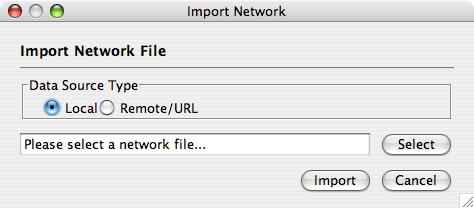
\includegraphics[width=\textwidth]{images/network_import_dialog1_25.png} 
\end{center}

\subsection{从远程计算机上导入网络(URL导入)}
在Import Networks中还可以使用URL导入网络文件。首先把Data Source Type设置成Remote,然后手动填写或是用书签插入合适的URL。点击文本域右边的箭头就能访问收藏的URL。(书签管理器的详细信息参阅Preferences中的Bookmark Manager一节。还可以把浏览器中的URL拖拽到URL文本框中。指定好URL后,点击Import按钮就能加载网络。

\begin{center}
 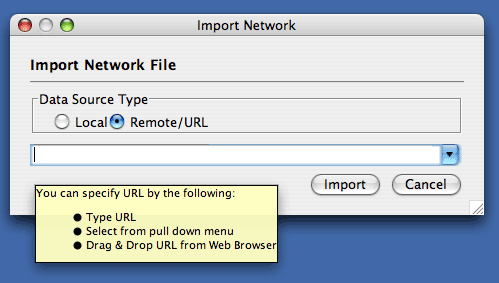
\includegraphics[width=\textwidth]{images/network_import_dialog2_25.png} 
\end{center}

从URL地址导入网络一定要注意一点。由于Cytoscape主要(但不是完全)是根据文件的后缀来判断文件的类型,所以如果URL中的文件的后缀不合适的话,在导入网络时就有可能遇到麻烦。如果Cytoscape没能在URL识别出有意义的文件名和后缀,它就会根据MIME类型来猜测文件的类型。如果所有的导入句柄就无法识别MIME类型,导入就会失败。

在导入网络时有可能遇到的另一个问题就是防火墙,导致无法访问文件。为了解决这个问题,Cytoscape支持使用代理服务器。在 Edit $\rightarrow$ Preferences$\rightarrow$ Proxy Server...中就可以设置代理服务器。在Preference有这方面的更多信息。

\section{导入格式灵活的表格文件}
从2.4版开始,Cytoscape就能通过Edit $\rightarrow$ Import $\rightarrow$ Network from Table (Text/MS Excel)...从文本文件和Excel文件中导入网络。在弹出的窗口中可以设置处理文件的各种选项。还能预览当前设置对文件的处理结果。修改设置时,预览窗口也会自动更新。除了设置文件的处理方法,用户还必须指定Source节点和Target节点,还可以这是边的类型。

\begin{center}
 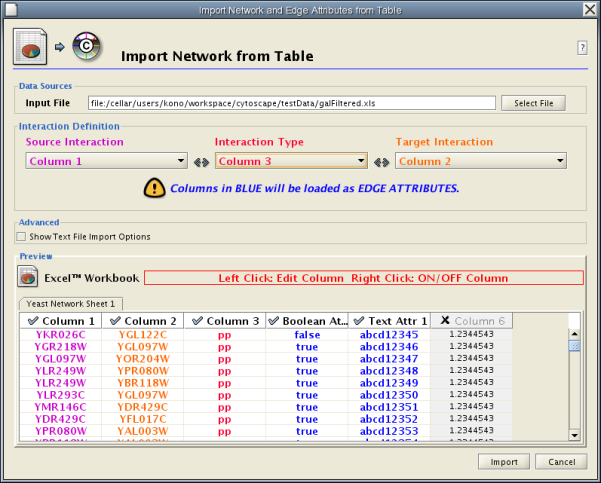
\includegraphics[width=\textwidth]{images/network_table_import.png} 
\end{center}

\subsection{支持的文件类型}
``Import Network from Table''功能支持按特定符号分割的文本文件,和单工作表的微软Excel文件。下面就是一个例子:

\medskip

{\tiny
\begin{tabular}{cccccc}
source  &target&  interaction&  boolean attribute&  string attribute&        floating point attribute\\
YJR022W &YNR053C &pp     & TRUE  &  abcd12371    &   1.2344543\\
YER116C &YDL013W &pp     & TRUE   & abcd12372    &   1.2344543\\
YNL307C &YAL038W &pp     & FALSE  & abcd12373    &   1.2344543\\
YNL216W &YCR012W &pd     & TRUE   & abcd12374    &   1.2344543\\
YNL216W &YGR254W &pd     & TRUE   & abcd12375    &   1.2344543
\end{tabular}}


网络文件至少要有两列:一列是起点,一列是终点。相互作用的类型是可选的。所以,最简单的网络表格应该是这样的:

\begin{verbatim}
YJR022W YNR053C
YER116C YDL013W
YNL307C YAL038W
YNL216W YCR012W
YNL216W YGR254W
\end{verbatim}

在网络文件中,每一行都是一条边以及这条边的属性。所以,网络文件是网络数据和边属性的组合。当然,表中的某些列可能并不是边的属性。遇到这种情况,就可以选择不导入这些列,在预览窗口中点击这一列的表头就是了。例如,在导入下面这种表时,这个功能有很有用:

\begin{verbatim}

Unique ID A  Unique ID B  Alternative ID A
Alternative ID B  Aliases A Aliases B Interaction
detection methods   First author surnames   Pubmed
IDs   species A species B Interactor types  Source
database Interaction ID  Interaction labels
Cross-references  Associated Files  Experiment
files  Experiment labels Different techniques
Different Pubmed articles Different sources Weight

7205 5747 TRIP6   PTK2 Q15654  Q05397-1  vv|HPRD
Currently not available
14688263|15892868(Marcotte)  Mammalia  Homo
sapiens protein|protein HPRD|Marcotte   0 Thyroid
hormone receptor interactor 6-FAK-|PTK2-TRIP6
NA(HPRD)|NA(Marcotte)
HPRD/02859_psimi.xml|other/ORIGINAL_DATA_MARCOTTE.txt
vv(HPRD/02859_psimi.xml)|HPRD(other/ORIGINAL_DATA_MARCOTTE.txt)
17651(ExptRef)|Marcotte 2 2 2 2

4174 7311 MCM5 UBA52   P33992  P62987
neighbouring_reaction   Currently not available
15608231(Reactome)   Homo sapiens Homo sapiens
protein|protein Reactome  1 P33992-P62988
Reaction:68944<->Reaction:68946(Reactome)|Reaction:68946<->
Reaction:68944(Reactome) other/ORIGINAL_DATA_MARCOTTE.txt
neighbouring_reaction(other/REACTOMEhomo_sapiens.interactions.txt)
Reactome 1 1 1 1

7040 7040 TGFB1   TGFB1   P01137  P01137  nmr:
nuclear magnetic resonance Currently not available
8679613 Homo sapiens Homo sapiens protein|protein
BIND 2 TGFB1-TGFB1- 72085(BIND)
BIND/bind_taxid9606.1.psi.xml   nmr: nuclear
magnetic resonance(BIND/bind_taxid9606.1.psi.xml)
NotAvailable 1 1 1 1

\end{verbatim}

这份数据是用制表符分割的,含有网络数据(相互作用)、边的属性和节点属性。把这份数据导入到~Cytoscape~中,首先选择~Unique ID A~作为起点,Unique ID B~作为目标,Interactor type作为相互作用类型。不要导入节点属性(ALternative ID A、species B等等)。其它的列则作为边的属性导入。

网络导入功能无法导入节点属性,只能导入边属性。关于节点属性的导入,请阅读本手册的~Attributes~一节。


注意:
\begin{enumerate}
	\item 这里的数据来自Andrew Garrow、Yeyejide Adeleye~和~Guy Warner(Unilever, Safety and Environmental Assurance Center, 2006年10月12日)的\emph{A merged human interactome}~数据集。在\url{http://www.cytoscape.orghttp://cytoscape.org/cgi-bin/moin.cgi/Data\_Sets/}上可以下载到真实的数据。
\end{enumerate}

\subsection{基本操作}

导入文本表格或Excel表格中的网络,步骤如下: 
\begin{enumerate}
\item 点击~File $\rightarrow$ Import $\rightarrow$ Network from Table (Text/MS Excel)... 
\item 点击~Select File~按钮,选择一份表格。 
\item 从表格中选择相互作用的起始点和相互作用类型。如果将相互作用的类型设置为缺省类型,则所有的相互作用的类型都会被设为pp;这个参数可以再Advanced Options中修改(下面会介绍)。
\item (可选)如果需要的话,可以定义边属性列。在表格中,除了网络数据,还可以有一些列来表示边的属性。
\begin{itemize}
\item 激活或取消属性列——在预览表格中鼠标左键单击表头,就能激活或去表边的属性。如果表头及该列的内容时蓝色的,则该列将会作为边的属性导入。例如,下面表格中的第1到第3列将会作为网络数据,第4列不会导入,而第5、6两列则会作为边属性导入。
\begin{center}
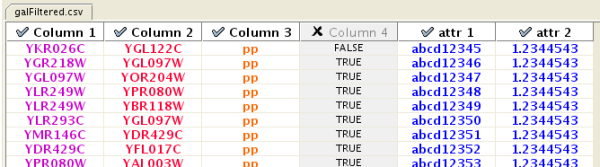
\includegraphics[width=.8\textwidth]{images/network_table_sample.png} 
\end{center}
\item 改变属性名称和数据类型——在预览表格的表头上用鼠标右键单击,就能修改属性的名称和数据类型。有关信息,详见下面的``修改属性名称和类型''。
\end{itemize}
\item 点击~Import按钮。 
\end{enumerate}

\subsection{导入不带边的节点列表}
在~Table Import~中可以导入不带边的节点列表。 如果只选择源节点列,就会创建一个没有相互作用的网络。在使用一些web服务客户端来扩展节点时,这个功能很有用。详细信息,请参阅``从外部数据库中导入网络''。

\subsection{高级选项}
\begin{center}
 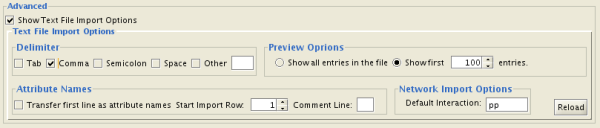
\includegraphics[width=\textwidth]{images/network_import_advanced.png} 
\end{center}
选择~Show Text File Import Option~选项,可以对一些选项进行设置。
\begin{itemize}
\item 分隔符(Delimiter):可以为文本表格选择多个分隔符。缺省情况下,分隔符是制表符和空格。
\item 预览选项(Preview Options):选好网络表格文件后,文件中的前一百行数据会显示在预览窗口中。修改这个选项的值,可以在预览窗口中显示更多的内容。如果要显示文件中所有的内容,选上``Show all entries in the file''即可。点击~Reload~按钮可以更新预览窗口中的内容。
\item 属性名称(Attribute Names)
\begin{itemize}
\item 将第一行设为属性名称(Transfer first line as attribute names):选上这个选项,所有的边的属性就会根据表格第一行命名。
\item 起始导入行(Start Import Row):设置从表格中第几行开始导入。例如,如果要忽略文件中的前三行,就可以将这个选项设为4。
\item 注释行(Comment Line:):以该字符开头的行将被视为注释,不会导入。这个选项可以用于跳过文件中的注释。
\end{itemize}
\item 网络导入选项(Network Import Options):如果相互作用的类型被设为缺省相互作用,所有边的类型就会被设为这个值。
\end{itemize}
 
\subsection{修改属性名称和类型}

\begin{center}
 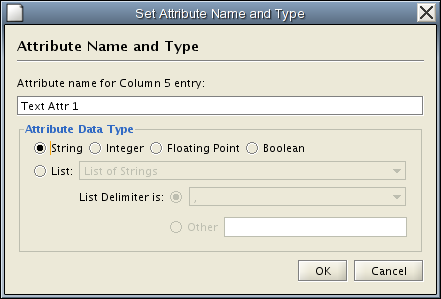
\includegraphics[width=\textwidth]{images/network_table_attr_dialog1.png} 
\end{center}

在这里可以修改属性的名称和数据类型。
\begin{itemize}
\item 修改属性名称(Modify Attribute Name):输入新的属性名称,然后点击OK即可。
\item 修改属性数据类型(Modify Attribute Data Type):支持以下数据类型:
\begin{itemize}
\item String 
\item Boolean (True/False) 
\item Integer 
\item Floating Point 
\item List of (one of) String/Boolean/Integer/Floating Point 
\end{itemize}
\end{itemize}
Cytoscape~有基本的数据类型探测功能,能自动地根据该列数据的内容推测数据的类型。不过还是可以自行选择合适的数据类型。对于list,必须要设置一个全局的分隔符(例如,表格中所有的单元格都必须使用相同的分隔符)。

\section{从~Web~服务导入网络}
从~2.6.0~开始,Cytoscape~有了一个新功能\textbf{Web Service~客户端管理器(Web Service Client Manager)}。有了这个功能,用户可以访问各种类型的数据库。
详见\emph{\textbf{从外部数据库导入网络和属性}}。

\section{编辑新网络}
在Cytoscape中还可以新建空网络,然后手动地添加节点和边。点击~File $\rightarrow$ New $\rightarrow$ Network $\rightarrow$ Empty Network,然后可以用CytoPanel 1中的Editor手动的添加网络节点和边(详见Editor一章)。
